\chapter{Introduction}
\label{chap:intro}

\makeatletter
\newenvironment{chapquote}[2][2em]
{\setlength{\@tempdima}{#1} \def\chapquote@author{#2} \parshape 1
  \@tempdima \dimexpr\textwidth-2\@tempdima\relax \itshape}
{\par\normalfont\hfill--\
\chapquote@author\hspace*{\@tempdima}\par\bigskip}
\makeatother

\begin{chapquote}{Morgan Freeman in {\em Transcendence (2014 film)}}
  ``Geo-locating suspects in real time? I've never seen anything like
it.''
\end{chapquote}

The ultimate goal of image understanding is to transfer visual
signals (images/videos) into abstract symbolic descriptions of the
world which are helpful for decision making.
However, understanding images is not a trivial task for machines.
In order to handle various complicated scenarios, researchers divide
image understanding into different computer vision tasks: pedestrian
detection for autonomous driving, face recognition for security
systems, and image retrieval for search engines.

For many applications, knowing when, where, and in which direction a
picture was taken is important scene understanding. However, most
images do not carry such information. 
We refer to the task of estimating this information as {\em
geo-calibration}. Our thesis focuses on developing geo-calibration
algorithms.

Most recent geo-calibration algorithms are deterministic
systems~\cite{baatz2012large,doersch2012what,li2012worldwide,kendall2015convolutional}.
Deterministic systems have some obvious drawbacks: 1) they cannot
model the inherent uncertainties from images of ambiguous scenes, and
2) without a proper modeling of the uncertainty, the subsequent
process can yield overly confident predictions. To address these
problems, we propose to build probabilistic systems for camera
geo-calibration.

We also show that learning to geo-calibrate a camera allows us to
learn about the scene of the image.
As an essential part of understanding the scene, how to extract image
features is an important problem has been studied for decades.  In
recent years, learning based approaches for image feature extraction
like convolutional neural networks have drawn a lot of attention due
to the fact that they do not need expert knowledge about the target
data. However, most of these feature learning methods require a large
quantity of manually labeled datasets. In this thesis, we propose
alternative ways to learn image features when the
manually labeled data is either insufficient or absent.

\section{Background}
To give a better understanding of our work, we would like to introduce
some related computer vision concepts before we discuss the main topics.
We start with the definition of geo-calibration,
along with its literature. Next, we introduce the history of deep
learning methods for geo-calibration, and data-driven scene matching
approaches that use aerial imagery. In the end, we cover some related
work of weakly supervised learning techniques.

\subsection{Geo-Calibration of Outdoor Images}
Automatic geo-calibration of outdoor images continues to grow in
importance as a direct result of the increasing amount of imagery
available via the Internet. Solving this problem is of great value
for a wide variety of fields, with potential applications ranging from
the forensic sciences~\cite{stylianou13jane} to environmental
monitoring~\cite{zhang2012mining}. Conceptually, the geo-calibration
task includes identifying the camera pose ({\em pose estimation}),
the camera geographic location ({\em geo-localization}), and the time
when the image was captured ({\em time estimation}).

\begin{itemize}[noitemsep]

\item \textbf{Pose Estimation:}
Pose estimation is to estimate the camera yaw, pitch, and roll
angles, $(\theta_{yaw}, \theta_{pitch}, \theta_{roll})$ from an
image. In the context of geo-calibration, the yaw angle
$\theta_{yaw}$ is referred to as the geographic orientation angle of
the camera.
%
Li et al.~\cite{li2012worldwide} exploit geo-registered 3D points
clouds to estimate camera pose.
Vo \etal~\cite{vo2016localizing} propose a geo-localization network
that can regress the geo-orientation angle of the camera.
Agarwal \etal~\cite{agarwal2015metric} keep track of the camera pose
changes by matching SIFT~\cite{lowe1999object} feature points detected
between the input image and Google Street View panoramas.
%
Horizon line detection is an essential step for some pose
estimation algorithms, because horizon lines are closely related to
camera pitch and roll angles.
Collins and Weiss~\cite{unitsphere1990} formulate horizon line
detection as a statistical estimation problem on the Gaussian Sphere.
More recent work has explored the use of dual
space~\cite{alignment2014,dualspace2013} representations. Among the
clustering-based approaches, Xu et al.~\cite{kitware2013} improve this
pipeline by introducing a new point-line consistency function that
models errors in the line segment extraction step.
\newline

\item \textbf{Geo-Localization:}
The task of geo-localization estimates the geographic location, $(lat,
lon)$, of the camera given image/video inputs.
%
As an important step of geo-localization, extracting
location-dependent features from image data has drawn a great detail
of attention from the vision community~\cite{jacobs07geolocate,
jacobs11geolocate, jacobs08geoorient}. The common trend amongst these
methods is that they take advantage of a large dataset of
geo-referenced images. Hays and Efros~\cite{hays2008im2gps} use a
data-driven scene matching approach to localize a query image using a
large dataset of geo-tagged images.  Doersch
\etal~\cite{doersch2012what} extract location-dependent features that
capture the relative appearance differences of large cities.  Lin et
al.~\cite{lin2013cross} localize a ground-level image by learning the
relationship between pairs of ground and aerial images \footnote{In
the context of our thesis, we do not distinguish between satellite
imagery and aerial imagery} of the same location. Other techniques
focus on urban environments and infer location using local image
descriptors~\cite{schindler2008detecting,snavely2006photo}.  Many
other cues exist, such as the
skyline~\cite{baatz2012large,ramalingam2009geolocalization}, sky
appearance~\cite{lalonde2010sun,workman2014rainbow}, and
shadows~\cite{junejo2008estimating,wu2010geo}.
\newline

\item \textbf{Time Estimation:}
The goal of time estimation is to estimate the time when the 
image was captured. Depending on the application, the accuracy of
predictions range from hour to year.
%
Matzen and Snavely~\cite{matzen2014scene} predict
timestamps for photos by matching against a time-varying
reconstruction of a scene.  Hill \etal~\cite{hill1994elephant} estimate the
time of the day by measuring the light intensity profiles captured by
cameras. Methods are proposed to date
yearbook photos by analyzing human
appearance~\cite{salem2016face2year,ginosar2015century}. Lee
\etal~\cite{linking2015iccp} find visual patterns in buildings,
relate them to certain time periods.
\newline

\end{itemize}

In conclusion, most of the geo-calibration algorithms we mention above
rely on finding visual cues from input images. To extract useful
visual features, a majority of these algorithms require strong human
expertise about the data, thus, they can only be applied in limited
scenarios. Therefore, we contribute to developing geo-calibration
algorithms without the need of strong human expertise about the data.

\subsection{Deep Learning in Geo-Calibration}
In recent years, deep neural networks (DNNs) were proven to be
extremely successful in many computer vision areas. 
It is widely accepted that DNNs have excellent performance in
high-level visual feature learning.
This valuable ability provides researchers powerful tools to
solve the challenging geo-calibration tasks.
Weyand and Kostrikov \etal~\cite{planet} propose a convolutional
neural network (CNN) to predict the geographic location of the input
image. Walch \etal~\cite{walch2017image} aggregate learned CNN
features with LSTM to generate global image representation for camera
localization.  Studies about camera pose
estimation~\cite{zhai2016horizon, workman2016horizon,
hold2017perceptual} have been done by identifying the horizon line with
CNNs (one can derive the camera roll and pitch angles from the horizon
line position giving the camera focal length).

Closely related to camera geo-calibration, problems of identifying
camera intrinsics using deep neural networks have also been studied.
Workman \etal~\cite{workman2015deepfocal} develop a CNN to estimate
the camera focal length. Kendall \etal~\cite{kendall2015convolutional}
propose a neural network that can identify 6-DOF camera parameters for
specific scenes.

All these geo-calibration methods share the common property that they
make the predictions directly out of DNNs. Besides these methods,
there exists another big category of methods that geo-calibrate
cameras using aerial imagery as geo-registered database. We will
discuss them in the following section.

\subsection{Ground-to-Aerial Geo-Calibration}
Data-driven scene matching approaches are commonly used in
geo-calibration.
When localizing a camera, data-driven algorithms search for k-nearest
neighbors of the query image in a database of the geo-tagged imagery.
To reduce the work of querying, the searching process is usually
carried out in a feature space of an applicable number of  
dimensions~\cite{im2gps, li2010location,zamir2010accurate}.
However, due to limited accuracies of GPS signals and the biased
distribution of human population, geo-tagged ground-level images
collected from smart devices are usually noisy and sparse in
geographic space. To achieve better geo-calibration results, we
need alternative image resources with more accurate geographic tags
and more complete spatial coverage.

Benefiting from the fast-growing monitoring satellite and drone markets,
geo-tagged aerial imagery has become more publicly accessible
than ever. Aerial imagery downloading service like
Microsoft Bing Map provides aerial images of various
resolutions, which cover most areas of the world with accurate
geographic registration, making aerial imagery a rich source for
reference databases. We refer to geo-calibration
methods which use the aerial imagery for geographic reference as
ground-to-aerial geo-calibration. Data used for ground-to-aerial
geo-calibration is referred to as cross-view pairs.
A cross-view pair consists of a ground image and an aerial image at
the same location (sometimes aligned in orientation).

Recent work on ground-to-aerial
geo-calibration~\cite{lin2013cross,lin2015learning,workman2015geocnn,workman2015wide}
has shown that convolutional neural networks are efficient for extracting
features from geo-tagged aerial imagery that can be matched to
features extracted from the ground imagery.  Vo
\etal~\cite{vo2016localizing} extend this line of work, demonstrating
improved geo-localization performance by applying an auxiliary loss
function to regress the ground-level camera orientation with respect
to the aerial image. Hu and Feng \etal~\cite{mh2018cvm} achieve the
state-of-the-art performance in geo-localization by extracting
cross-domain global features using the
NetVLAD~\cite{arandjelovic2016netvlad} technique.

The key for the success of these methods is to learn descriptive
features for ground-to-aerial imagery matching. In the following
section, we will introduce literature about feature learning techniques.

\subsection{Feature Learning with Weak Annotations}

Manually engineering visual features is a common practice for
computer vision tasks. One of successful examples of manual
feature is SIFT~\cite{lowe1999object}, which is widely used by many
computer vision algorithms.
In recent years, automatic feature engineering has drawn more
attention. Compared to the manual feature
engineering, automatic feature engineering allows to learn
useful features with much less (if not none) knowledge about the data.
Among these learning approaches, deep neural networks are intensively
studied.  The most common approach for deep feature learning is full
supervision, which usually requires a large number of manual
annotations~\cite{yosinski2014transferable,zhou2016learning,wen2016discriminative}.
Unfortunately, such data is not always available for certain tasks or
requires a huge amount of human labor. 
In contrast, unlabeled data is often plentiful (\ie cellphone photos in Instagram
or Youtube videos).

To lavage these unlabeled data, recent work has explored
self-supervision methods (sometimes referred to as unsupervised learning or
pretext tasks) for training deep neural networks that capture useful
visual representations~\cite{doersch2015unsupervised,pathak2016context}. 
These methods typically
exploit some known quantity of the data, like pixel color values, to
avoid expensive manual annotation.
By learning these quantities associated with the data, one
can obtain useful features of the image.
For example, Zhang et al.~\cite{zhang2016colorful} show how
synthesizing colors for a grayscale image is a powerful
pretext task for learning visual representations. Pathak et
al.~\cite{pathak2017learning} exploit low-level motion-based grouping
cues for unsupervised feature learning.  
%
As one of new learning techniques that address the lack of massive amounts
of labeled data, domain adaptation forces the feature generating model
to adapt another feature domain so that it improves the performance
when dealing with new input
data~\cite{fernando2013unsupervised,fernando2015joint,saenko2010adapting,wang2016actions,tinghui2016flow}.
Duan \etal~\cite{duan2012learning} propose to learn a linear
projection to transfer from the source feature subspace to the target
subspace. Sohn \etal~\cite{sohn2017unsupervised} improve the
performance of video face recognition using an adversarial-based
approach to adapt the network to unlabeled video imagery.

We have explained four related computer vision concepts so far. In the
following section, we are going to discuss our main contributions.

\section{Main Contributions}

\begin{figure}
  \centering
  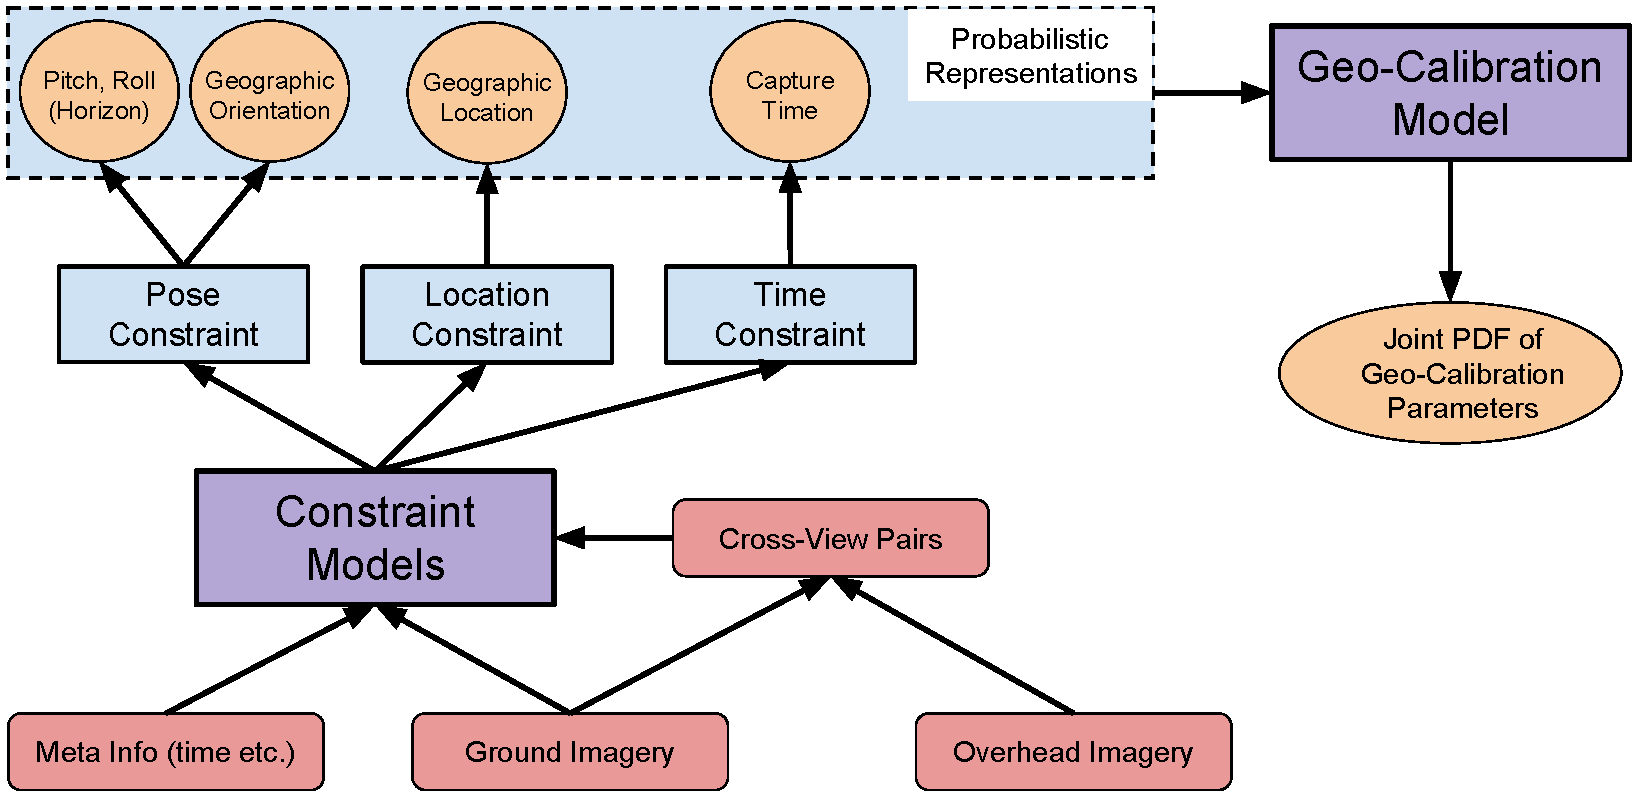
\includegraphics[width=\linewidth]{introduction/architecture}
  \caption{A simplified flowchart of our approach. The algorithm
inputs (images, time and manual annotations) are fed to different
constraint models which work as constraint functions. 
The probabilistic distribution over complete geo-calibration
parameters are then simulated jointly by fusing these constraint
functions in a general model for geo-calibration.}
  \label{fig:intro:architecture}
\end{figure}

We make contributions in three main areas: 1) we
proposed a reflexible probabilistic model to jointly estimate the
geo-calibration parameters, 2) we decomposed the full geo-calibration
into several partial geo-calibration tasks, each of which provides a
strong constraint function that fits into the probabilistic model,
and 3) we show that learning to geo-calibrate a camera is a useful
pretext for image feature learning.
 
The first two contributions make our main approach. Our
algorithm feeds inputs (images, time, and manual annotations) to
different constraint functions, which we can fuse together to simulate
the joint distribution over the complete geo-calibration parameters.
We present the flowchart of our approach in
\figref{intro:architecture}.
%
Furthermore, based on the belief that the content of the image is usually dictated
by the camera pose, geographic location and image capture time. We
treat geo-calibration information as pretext task and show that they
are useful for image feature learning.


\subsection{Flexible Probabilistic Model for Geo-Calibration}
We design a flexible probabilistic model to estimate the probability
over all geo-calibration parameters.
First, we construct a scoring function to model the process of camera
projecting the scene to image frame at given pose, location, and time.
%
The scoring function measures the ``fitness'' between these
geo-calibration parameters and the appearance of the image. 
It consists of a series of constraint functions,
%
The scoring function is proportional to the probability distribution
over the geo-calibration parameters. Since the integral over all
possible parameters is intractable, we propose a Markov Chain Monte
Carlo (MCMC) sampling approach to approximate the underlying
probability distribution. 
%
Our model is flexible because it allows different constraint functions
contribute to the scoring function. The details of this model can be
found in \chapref{mcmc}.

\subsection{Developing Constraint Functions}
The scoring function of the probabilistic
model is defined as a weighted summation of a series of constraint
functions.
A constraint function outputs a score (or probability) of the input
geo-calibration parameters given the input image. In the rest of the
work, we focus on developing good constraint functions for different
sets of geo-calibration parameters. 

\begin{itemize}[noitemsep]
  \item \textbf{Constraint for Camera Pose:}
  We build the constraint function for camera roll and pitch angles.
  Assuming the intrinsic parameters are known, camera roll and pitch
  angles can be derived from the horizon line position on the image.
  Compared to directly detecting the camera pose, identifying the horizon
  line is easier because it can be explicitly estimated from the scene
  layout.
  In our work, we create a convolutional neural network to estimate the
  prior distribution over the horizon line.
  For each horizon line candidate sampled from the prior distribution,
  we assign a consistency score to it by measuring the consistencies of
  vanishing points detected on it.
  The constraint function output is defined as the multiplication of
  the prior probability of the associated horizon line and its
  consistency score.
  We present the algorithm details in \chapref{fasthorizon}.
  \newline

  \item \textbf{Constraint for Time and Location:}
  In this work, we estimate the probability over 
  the camera geographic location and the capture time of the input
  image.
  Our network has two branches that predict the image
  capture time and the geographic location simultaneously.
  For time estimation, our network is able to predict the
  joint distribution over the month of the year and the UTC hour of the
  day when the input image was captured.
  For camera geo-localization, our network outputs the discrete
  distribution over the geographic location of the camera. Better
  results can be procured with the image capture time as auxiliary input
  (if it is known).  
  We present the algorithm details in \chapref{whenwhere}.
  \newline

  \item \textbf{Constraint for Location and Orientation:}
  The previous algorithm only estimates locations approximately
  due to the limited capacity of the deep neural network. In this
  work, we propose a ground-to-aerial geo-calibration method that can
  further refine the prediction results and estimate the
  camera geo-orientation.
  %
  We designed a network that can jointly learn the semantic layout of
  the aerial image and its projection to the ground-level perspective.
  When computing the value of the constraint function, we feed the aerial
  image of a given location and orientation to the network. 
  By comparing the aerial-to-ground layout with the real layout of the
  ground image, we are able to measure the consistency between the two
  and use it as the value of our constraint function.
  We present the algorithm details in \chapref{crosstransf}.
  \newline

\end{itemize}


\subsection{Geo-Calibration for Feature Learning and Image
Understanding}
Full supervision algorithms are powerful tools to learn useful image
features. However, full supervision algorithms require large number
of annotated data, which takes a lot of human labor and is usually
unavailable.
On the other hand, images with annotations like tags and GPS locations
uploaded by individual users or captured automatically by smart
devices are plentiful on the Internet.
To use these image resources to understand the world,
we explore two approaches that use time and
locations as weak annotations: 1) {\em ground-to-aerial segmentation}, and 2)
{\em geo-temporal feature learning} with time/location tagged images.
 
\begin{itemize}[noitemsep]
  \item \textbf{Ground-to-Aerial Segmentation:}
  Semantic segmentation plays an important role in image understanding.
  The training for semantic segmentation tasks require a large number
  of annotated data.
  However, most large scale annotated datasets like ImageNet~\cite{ILSVRC15}
  and COCO~\cite{lin2014microsoft} are mostly made of ground-level
  images. By comparison, annotated datasets for aerial imagery are rare.
  %
  To deal with this problem, we proposed a
  DNN to learn semantic segmentation for aerial images with only
  ground-level annotations. Our method exploits the spatial
  correspondences between images in the cross-view pair, where the
  aerial imagery and ground imagery are associated by location and
  geo-orientation.
  In this work, we transfer the semantic knowledge from the
  ground domain to the aerial domain by identifying their latent
  geometric correspondences. Similar to {\em
  Reprojection Losses}~\cite{garg2016unsupervised,
  godard2017unsupervised,zhou2017unsupervised, yan2016perspective},
  which are proven to be successful in monocular depth estimation,
  our network learns the geometric projection from aerial to ground, and
  to semantically segment the aerial images jointly.
  We present the learning details in \chapref{crosstransf}
  \newline

  \item \textbf{Location and Time as Pretext Task:}
  Smart devices like cellphones and webcams get more sophisticated
  nowadays. Most of them are equipped with clocks and GPS modules. Thanks to
  the development of social networks, researchers now can find
  large amount of images online that are tagged with time and
  geographic locations. In \chapref{whenwhere}, we propose an
  algorithm that treats the location and time as pretext tasks to learn
  useful image features.  By learning to predict the geographic location
  and the capture time of the query image, our network learns to extract
  geo-temporal features from the image.

\end{itemize}

In summary, the main contributions of our work include developing a
probabilistic framework to solve geo-calibration problems, and
proposing new methods to learn image features with geo-calibration
information. We are going to present our approaches in detail in the
following chapters.
